\documentclass[11pt,a4paper]{article}
\usepackage[hyperref]{acl2018}

\usepackage{times}
%\usepackage[author={Lyndon}]{pdfcomment}
\usepackage{url}
%\usepackage[subtle]{savetrees}

%%%%%%%%%%%
%Graphics
\usepackage{graphicx}
\usepackage{tikz}
\usetikzlibrary{positioning,arrows,shapes,fit,  shapes.geometric}
\tikzset{
	every picture/.style={/utils/exec={\sffamily}},
	every matrix/.style={ampersand replacement=\&, rounded corners=10pt},
	every node/.style = {font=\small, inner sep = 3},
	>=latex,
	every text node part/.style={align=center}, auto,node distance=2.4, ->,
	every edge/.append style={every node/.style={font=\footnotesize}}
}
\usepackage[subpreambles=false]{standalone}

%%%%%%%%%%%
%  Tables
\usepackage{booktabs}
\usepackage{pgfplotstable}
\pgfplotsset{compat=1.14}



\pgfplotstableset{col sep=comma, header=has colnames,
%	numcol/.style={},
	string replace={"}{},
	string replace={ASIAF}{ASOIAF},
	string replace={ASOIAF+SOC}{\small ASOIAF+SOC},
	string replace={WOT+ASOIAF}{\small WOT+ASOIAF},
	string replace={WOT+SOC}{\small WOT+SOC},
%	string replace={Features}{\small Feats.},
	string replace={Most Commonly Mentioned}{Most Mentioned},
	numeric type, precision=3, fixed zerofill=true, fixed,
	%			bf content/.style={postproc cell content/.style={@cell content/.add={1\textbf{##1}}}},
	stringcol/.style={string type, column type={r}},
	%
	columns/Train Set/.style={stringcol},
	columns/Test Set/.style={stringcol},
	columns/Dataset/.style={stringcol},
	columns/Method/.style={stringcol},
	%
	every head row/.style={after row = {\toprule}}
}


%%%%%%%%%%%%%%%%%%%
% Math 

\usepackage{amssymb}
\usepackage{amsmath}
\usepackage{mathtools}
\DeclareMathOperator*{\argmin}{arg\,min}
\DeclareMathOperator*{\argmax}{arg\,max}

\newcommand{\compactmath}[1]{\noindent\resizebox{\columnwidth}{!}{$#1$}}
%%%%%%%%%%%%%%%%%%%%%%%%
\usepackage{cleveref}

%%%%%%%%%%%%%%%%%%%%%%%%%%%%%%%%%%%%
\usepackage{natbib}
\bibliographystyle{apalike}

\newcommand{\parencite}{\citep}
\newcommand{\textcite}{\cite}


%opening
\title{NovelPerspective: Identifying Point of View Characters}
\author{Lyndon White, %
	Roberto Togneri, %
	Wei Liu, %
	\and Mohammed Bennamoun%
	\\ 
	\url{lyndon.white@research.uwa.edu.au}, %
	\url{roberto.togneri@uwa.edu.au},\\
	\url{wei.liu@uwa.edu.au}, %
	\and \url{mohammed.bennamoun@uwa.edu.au}%
	\\
	The University of Western Australia.
	35 Stirling Highway, Crawley, Western Australia
}

\aclfinalcopy

\begin{document}

\maketitle

\begin{abstract}
We present NovelPerspective: a tool to allow consumers to subset their digital literature, based on point of view (POV) character.
Many novels have multiple main characters each with their own storyline running in parallel.
A well-known example is George R. R. Martin's  novel: ``A Game of Thrones'', and others from that series.
Our tool detects the main character that each section is from the POV of,
and allows the user to generate a new ebook with only those sections.
This gives consumers new options in how they consume their media; allowing them to  pursue the storylines sequentially, or skip chapters about characters they find boring.
We present two heuristic-based baselines, and two machine learning based methods for the detection of the main character.
\end{abstract}

\section{Introduction}
Often each section of a novel is written  from the perspective of a different main character.
The characters each take turns in the spot-light,
with their own parallel storylines being unfolded by the author.
As readers, we have often desired to read just one storyline at a time, particularly when reading the book a second-time.
In this paper, we present a tool, NovelPerspective, to give the consumer this choice.

Our tool allows the consumer to select which characters of the book they are interested in,
and to generate a new ebook file containing just the sections from that character's point of view (POV).
The critical part of this system is the detection of the POV character.
This is not an insurmountable task, building upon the well established field of named entity recognition.
However to our knowledge there is no software to do this.
Such a tool would have been useless, in decades past when booked were distributed only on paper.
But today, the surge in popularity of ebooks has opened a new niche for consumer narrative processing.
Methods are being created to extract social relationships between characters \parencite{elson2010socialnetworks,wohlgenannt2016extracting};
to align scenes in movies with those from books \parencite{moviebook}; and to otherwise augment the literature consumption experience.
Tools such as the one presented here, give the reader new freedoms in controlling how they consume their media.


Having a large cast of characters, in particular POV characters, is a hallmark of the epic fantasy genre.
Well known examples include: George R.R. Martin's ``A Song of Ice and Fire'', 
Robert Jordan's ``Wheel of Time'', Brandon Sanderson's ``Cosmere'' universe, and
Steven Erikson's ``Malazan Book of the Fallen'', amongst thousands of others.
Generally, these books are written in \emph{limited} third-person POV;
that is to say the reader has little or no more knowledge of the situation described than the main character does.

We focus here on novels written in the \emph{limited} third-person POV.
In these stories, the main character is, for our purposes, the POV character.
Limited third-person POV is written in the third-person, that is to say the character is referred to by name, but with the observations limited to being from the perspective of that character.
This is in-contrast to the \emph{omniscient} third-person POV, where events are described by an external narrator.
Limited third-person POV is extremely popular in modern fiction.
It preserves the advantages of first-person, in allowing the reader to observe inside the head of the character, while also allowing the flexibility to the perspective of another character \parencite{booth2010rhetoric}.
This allows for multiple concurrent storylines around different characters.
Our tool helps users un-entwine such storylines, giving the option to process them sequentially.


The utility of dividing a book in this way varies with the book in question.
Some books will cease to make sense when the core storyline crosses over different characters.
Other novels, particularly in epic fantasy genre,
have parallel storylines which only rarely intersect.
While we are unable to find a formal study on this, 
anecdotally many readers speak of:
\begin{itemize}
	\item ``Skipping the chapters about the boring characters.''
	\item ``Only reading the \emph{real} main character's sections.''
	\item ``Reading ahead, past the side-stories, to get on with the \emph{main} plot.''	
\end{itemize}
Particularly if they have read the story before, and thus do not risk confusion.
Such opinions are a matter of the consumer's personal taste.
The NovelPerspective tool gives the reader the option to customise the book in this way, according to their personal preference.

We note that sub-setting the novel once does not prevent the reader from going back and reading the intervening chapters if it ceases to make sense, or from sub-setting again to get the chapters for another character whose path intersects with the storyline they are currently reading.
We can personally attest for some books reading the chapters one character at a time is indeed possible, and pleasant: the first author of this paper read George R.R. Martin's ``A Song of Ice and Fire'' series in exactly this fashion.


The primary difficulty in segmenting ebooks this way is attributing each section to its POV character.
That is to say detecting who is the point of view character.
Very few books indicate this clearly, and the reader is expected to infer it during reading.
This is easy for most humans, but automating it is a challenge.
To solve this, the core of our tool is its character classification system.
We investigated several options which the main text of this paper will discuss.


\section{Character Classification Systems}

\begin{figure*}
	\resizebox{\textwidth}{!}{
		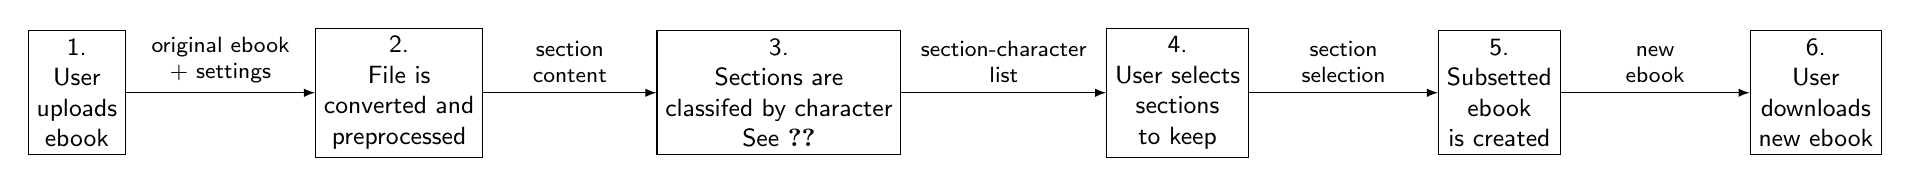
\begin{tikzpicture}		
		\node(start)[draw] {1.\\User\\ uploads\\ ebook};
		\node(convert)[draw, right=of start] {2.\\ File is\\ converted and \\preprocessed};
		\node(classify)[draw, right=of convert, xshift=-0.2cm] {3.\\Sections are \\ classifed by character\\ See \Cref{fig:classify}};
		\node(select)[draw, right= of classify, xshift=0.2cm] {4.\\User selects\\ sections\\ to keep};
		\node(create)[draw, right=of select] {5.\\Subsetted\\ ebook\\ is created};
		\node(download)[draw, right=of create] {6.\\User \\downloads \\ new ebook};
		
		\path (start) edge[below] node[above]{original ebook \\ + settings}  (convert);
		\path (convert) edge[below] node[above]{section\\ content} (classify);
		\path (classify) edge[below] node[above]{section-character\\list} (select);
		\path (select) edge[below] node[above]{section\\selection}  (create);
		\path (create) edge[below] node[above]{new \\ ebook}  (download);	
		\end{tikzpicture}
	}
	\caption{The full NovelPerspective pipeline. Note that step 5 uses the original ebook to subset. \label{fig:fullprocess}
	}
\end{figure*}

\begin{figure*}
	\resizebox{\textwidth}{!}{
		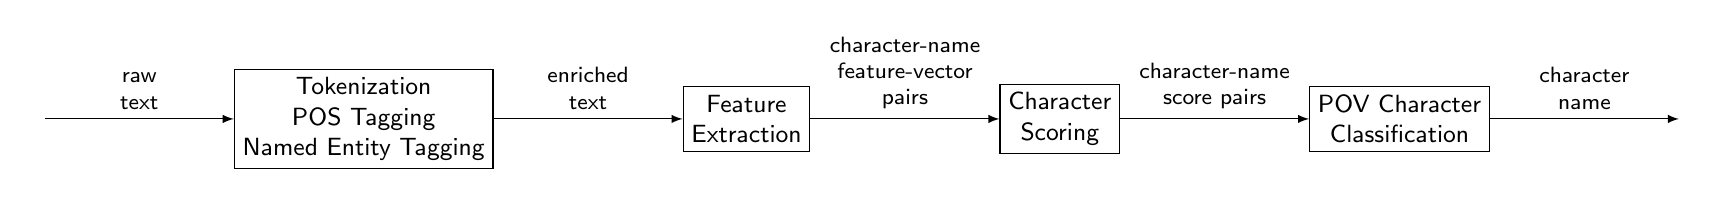
\begin{tikzpicture}		
		\node(start){};
		\node(enrich)[draw, right=of start] {Tokenization\\POS Tagging\\Named Entity Tagging};
		\node(features)[draw, right=of enrich] {Feature\\ Extraction};
		\node(scoring)[draw, right=of features] {Character\\Scoring};				
		\node(classify)[draw, right=of scoring] {POV Character\\ Classification};
		\node(end)[right=of classify] {};
		
		\path (start) edge node[above]{raw\\ text}  (enrich);
		\path (enrich) edge node[above]{enriched\\text} (features);
		\path (features) edge node[above]{character-name\\feature-vector\\pairs
		} (scoring);
		\path (scoring) edge node[above]{character-name\\score pairs
		} (classify);
		\path (classify) edge node[above]{character\\name}  (end);
		\end{tikzpicture}
	}
	\caption{The general structure of the character classification systems. This repeated for each section of the book during step 3 of the full pipeline shown in \Cref{fig:fullprocess}. \label{fig:classify}}
\end{figure*}

The full NovelPerspective pipeline is shown in \Cref{fig:fullprocess}.
The core character classification step (step 3), is detailed in \Cref{fig:classify}.
In this step the raw text is first enriched with parts of speech, and named entity tags.
We do not perform co-reference resolution, working only with direct entity mentions.
From this, features are extracted for each named entity.
These feature vectors are used to score the entities for the most-likely POV character.
The highest scoring character is returned by the system.
The different systems presented modify the \textbf{Feature Extraction} and \textbf{Character Scoring} steps.
A broadly similar idea, for detecting the focus location of news articles, was presented by \textcite{2017focus}.


\subsection{Baseline systems}
To the best of our knowledge no systems have been developed for this task before.
As such, we have developed two deterministic baseline character classifiers.
These are both potentially useful to the end-user in our deployed system (\Cref{sec:demonstration}),
and used to gauge the performance of the more complicated systems in the evaluations presented in \Cref{sec:results-and-discussion}.

It should be noted that the baseline systems, while not using machine learning for the character classification steps, do make extensive use of machine learning-based systems during the preprocessing stages.

\subsubsection{``First Mentioned'' Entity}
An obvious way to determine the main character of the section is to select the first named entity.
We use this to define the ``First Mentioned'' baseline
In this system, the \textbf{Feature Extraction} step is simply retrieving the position of the first use of each name;
and the \textbf{Character Scoring} step assigns each a score such that earlier is higher.
This works for many examples: \emph{``One dark and stormy night, Bill heard a knock at the door.''};
however it fails for many others: \emph{`` `Is that Tom?' called out Bill, after hearing a knock.'}'.
Sometimes a section  may go several paragraphs describing events before it even mentions the character who is perceiving them.
This is a varying element of style.

\subsubsection{``Most Mentioned'' Entity}
A more robust method to determine the main character, is to use the occurrence counts.
We call this the ``Most Mentioned'' baseline.
The \textbf{Feature Extraction} step is to count how often the name is used.
The \textbf{Character Scoring} step assigns each a score based what proportional of all names used were for this entity.
This works well for many books.
The more important a character is, the more often their name occurs.
However, it is fooled, for example, by book chapters that are about the POV character's relationship with a secondary character.
In such cases the secondary character may be mentioned more often.

\subsection{Machine learning systems}
One can see the determination of the main character as a multi-class classification problem.
From the set of all named entities in the section, classify that section as to which one is the main character.
Unlike typical multi-class classification problems
the set of possible classes varies per section being classified.
Further, even the total set of possible named characters, i.e.  classes, varies from book to book.
An information extraction approach is required which can handle these varying classes.
As such, a machine learning model for this task can not incorporate direct knowledge of the classes (i.e. character names).

We reconsider the problem as a series of binary predictions.
The task is to predict if a given named entity is the point of view character.
For each possible character (i.e. each named-entity that occurs), a feature vector is extracted (see \Cref{sec:feature-extraction-for-ml}).
This feature vector is the input to a binary classifier, which determines the probability that it represents the main character.
The \textbf{Character Scoring} step is thus the running of the binary classifier:
the score is the output probability normalised over all the named entities.



\subsubsection{Feature Extraction for ML}\label{sec:feature-extraction-for-ml}
We investigated two feature sets as inputs for our machine learning-based solution.
They correspond to different \textbf{Feature Extraction} steps in \Cref{fig:classify}.
A hand-engineered feature set, that we call the ``Classical'' feature set;
and a more modern ``Word Embedding'' feature set.
Both feature sets give information about how the each named entity token was used in the text.


The  ``Classical'' feature set uses features that are well established in NLP related tasks.
The features can be described as \emph{positional features}, like in the First Mentioned baseline; \emph{occurrence count features}, like in the \emph{Most Mentioned} baseline
and \emph{adjacent POS counts}, to give usage context.
The \emph{positional features} are the index (in the token counts) of the first and last occurrence of the named entity.
The \emph{occurrence count features} are simply the number of occurrences of the named entity, supplemented with its rank on that count compared to the others.
The \emph{adjacent POS counts} are the occurrence counts of each of the 46 POS tags on the word prior to the named entity, and on the word after.
We theorised that this POS information would be informative, as it seemed reasonable that the POV character would be described as doing more things, so co-occurring with more verbs.
This gives 100 base features.
To allow for text length invariance we also provide each of the base features expressed as a portion of its maximum possible value (e.g. for a given POS tag occurring before a named entity, the potion of times this tag occurred).
This gives a total of 200 features.




The ``Word Embedding'' feature set uses FastText word vectors \parencite{bojanowski2016enriching}.
We use the pretrained 300 dimensional embeddings trained on English Wikipedia \footnote{\url{https://fasttext.cc/docs/en/pretrained-vectors.html}}.
We concatenate the 300 dimensional word embedding for the word immediately prior to, and immediately after each occurrence of a named entity;
and take the element-wise mean of this concatenated vector over all occurrences of the  entity.
Such averages of word embeddings have been shown to be a useful feature in many tasks \parencite{White2015SentVecMeaning,mikolovSkip}.
This has a total of 600 features.

\subsubsection{Classifier}
The binary classifier, that predicts if a named entity is the main character, is the key part of the \textbf{Character Scoring} step for the machine learning systems.
From each text in the training dataset
we generated a training example for every named entity that occurred.
All but one of these was a negative example.
We then trained it as per normal for a binary classifier.
The score for a character is the classifier's predicted probability of its feature vector being for the main character.
%This idea of using the output of a binary classifier as a score has been used, for example, by \textcite{corston2001machine} where they rate machine translations using a binary classification probability of them being written by a human.

Our approach of using a binary classifier to rate each possible class,
may seem similar to the one-vs-rest approach for multi-class classification.
However, there is an important difference.
Our system only uses a single binary classifier; not one classifier per class,
as the classes in our case vary with every item to be classified.
The fundamental problem is information extraction, and the classifier is a tool for the scoring which is the correct information to report.


With the classical feature set we use logistic regression, with the features being preprocessed with 0-1 scaling.
During preliminary testing we found that many classifiers had similar high degree of success, and so chose the simplest.
With the word embedding feature set we used a radial bias support vector machine, with  standardisation during preprocessing,
as has been commonly used with word embeddings on other tasks.



\section{Experimental Setup}\label{sec:experimental-setup}
\subsection{Datasets}
We make use of three series of books selected from our own personal collections.
The first four books of George R. R. Martin's ``A Song of Ice and Fire'' series (hereafter referred to as ASOIAF);
The two books of  Leigh Bardugo's ``Six of Crows'' duology (hereafter referred to as SOC);
and the first 9 volumes of Robert Jordan's ``Wheel of Time'' series (hereafter referred to as WOT).
In \Cref{sec:results-and-discussion} we consider the use of each as a training and testing dataset.
In the online demonstration (\Cref{sec:demonstration}), we deploy models trained on the combined total of all the datasets.

To use a book for the training and evaluation of our system, we require a ground truth for each section's POV character.
ASOIAF and SOC provide ground truth for the main character in the chapter names.
Every chapter only uses the POV of that named character.
WOT's ground truth comes from an index created by readers.\footnote{\url{http://wot.wikia.com/wiki/List_of_Point_of_View_Characters}}
We do not have any datasets with labelled sub-chapter sections, though the tool does support such works.


\begin{table}
	\begin{tabular}{rcc}
		Dataset & Chapters & POV Characters\\
		\toprule
		ASOIAF  & 256	&	15\\
		SOC		& 91	&	9\\
%		SA		& 275	&	6\\
		WOT     & 432   &   52\\
		\midrule
		\textbf{combined}  &  779 & 76
	\end{tabular}
	\caption{The number of chapters and point of view characters for each dataset. \label{tbl:datasets}}
\end{table}

The total counts of chapters and characters in the datasets, after preprocessing, is shown in \Cref{tbl:datasets}.
Preprocessing consisted of  discarding chapters for which the POV character was not identified (e.g. prologues); and of removing the character names from the chapter titles as required.

\subsection{Evaluation Details}
In the evaluation, the systems are given the body text and asked to predict the character names.
During evaluation, we sum the scores of the characters alternative aliases/nick-names used in the  books.
For example merging \texttt{Ned} into \texttt{Eddard} in ASOIAF.
This roughly corresponds to the case that a normal user can enter multiple aliases into our application when selecting sections to keep.
We do not use these aliases during training, though that is an option that could be investigated in a future work.

\subsection{Implementation}
The implementation is available on GitHub.
\footnote{\url{https://github.com/oxinabox/NovelPerspective/}}
Scikit-Learn \parencite{scikit-learn} is used for the machine learning and evaluations,
and NLTK \parencite{NLTK} is used for textual preprocessing.
The text is tokenised, and tagged with POS and named entities using NLTK's default methods.
Specifically, these are the Punkt sentence tokenizer, the regex-based improved TreeBank word tokenizer, greedy averaged perceptron POS tagger, and the max-entropy binary named entity chunker.
The use of a binary, rather than a multi-class, named entity chunker is significant.
Fantasy novels often use ``exotic'' names for characters, we found that this often resulted in character named entities being misclassified as organisations or places.
Note that this is particularly disadvantageous to the First Mentioned baseline, as any kind of named entity will steal the place.
Nevertheless, it is required to ensure that all character names are a possibility to be selected.


\section{Results and Discussion}\label{sec:results-and-discussion}

\begin{table}
	\begin{adjustbox}{max width=\columnwidth}
		\pgfplotstableset{best/.append style={
				postproc cell content/.style={@cell content/.add={$\bf}{$}}
			},
		nearbest/.append style={
			postproc cell content/.style={@cell content/.add={$\it}{$}}
		}
	}
		
		\pgfplotstabletypeset[%
			every row 3 column Acc/.style={best},
			%
			every row 14 column Acc/.style={best},
			every row 15 column Acc/.style={best},
			%
			every row 19 column Acc/.style={best},
			%
			every nth row={8}{before row=\cmidrule{2-4}},
			]{results/maineval.csv}
	\end{adjustbox}
	
	\caption{The results of the character classifier systems. The best results are \textbf{bolded}.
	%Results that are within a single classification error of the best, are \textit{italicised}.
	} \label{tbl:resmain}
\end{table}

Our evaluation results are shown in \Cref{tbl:resmain} for all methods.
This includes the two baseline methods, and the machine learning methods with the different feature sets.
We evaluate the machine learning methods using each dataset as a test set, and using each of the other two and their combination as the training set.

The First Mentioned baseline is very weak.
The Most Mentioned baseline is much stronger.
In almost all cases machine learning methods outperform both baselines.
The results of the machine learning method on the ASOIAF and SOC are very strong.
The results for WOT are weaker, though they are still accurate enough to be useful when combined with manual checking.


It is surprising that using the combination of two training sets does not always out-perform each on their own.
For many methods training on just one dataset resulted in better results.
We believe that the difference between the top result for a method and the result using the combined training sets is too small to be meaningful.
It can, perhaps, be attributed to a coincidental small similarity in writing style of one of the training books to the testing book.
To maximise the generalisability of the NovelPerspective prototype (see \Cref{sec:demonstration}), we deploy models trained on all three datasets combined.

Almost all the machine learning models resulted in similarly high accuracy.
The exception to this is word embedding features based model trained on SOC, which for both ASOIAF and WOT test sets performed much worse.
We attribute the poor performance of these models to the small amount of training data.
SOC has only 91 chapters to generate its training cases from, and the word embedding feature set has 600 dimensions.
It is thus very easily to over-fit which causes these poor results.
%Using a different, lower dimensional set of pretrained word embeddings mould likely decrease this over-fitting, however given the existence of more data allowing other methods to fit we have not investigated this.


\begin{table}
	\begin{adjustbox}{max width=\columnwidth}
		\small
		\pgfplotstableset{best/.append style={
				postproc cell content/.style={@cell content/.add={$\bf}{$}}
			},
			nearbest/.append style={
				postproc cell content/.style={@cell content/.add={$\it}{$}}
			}
		}
		
		\pgfplotstabletypeset[%
		every nth row={2}{before row=\cmidrule{2-4}},
		]{results/traineval.csv}
	\end{adjustbox}
	
	\caption{The training set accuracy of the machine learning character classifier systems.
	} \label{tbl:restrain}
\end{table}

\Cref{tbl:restrain} shows the training set accuracy of each machine learning model.
This is a rough upper bound for the possible performance of these models on each test set, as imposed by the classifier and the feature set.
The WOT bound is much lower than the other two texts.
This likely relates to WOT being written in a style that closer to the line between third-person \emph{omniscient}, than the more clear third-person \emph{limited} POV of the other texts.
We believe longer range features are required to improve the results for WOT.
However, as this achieves such high accuracy for the other texts, further features would not improve accuracy significantly, without additional more difficult training data (and may cause over-fitting).

%
%The word embedding feature set only contains context information, not frequency information, but still performs well.
%Further, it only uses a single word window to each side of the named entity.
%This suggests that the point of view character can largely be inferred only from the usage of its name. 
%This is in-line with a human's ability to read an arbitrary paragraph and identify the point of view character.
%
The results do not show a clear advantage to either machine learning feature set.
Both the classical features and the word embeddings work well.
Though, it seems that the classical feature are more robust; both with smaller training sets (like SOC), and with more difficult test sets (like WOT).

\section{Demonstration System}\label{sec:demonstration}
We have deployed an online prototype to \url{https://white.ucc.asn.au/tools/np}.
A video of its use can be found at \url{https://youtu.be/iu41pUF4wTY}.
This web-app, made using the CherryPy framework,\footnote{\url{http://cherrypy.org/}}
allows the user to apply any of the model discussed to their own novels.

The web-app functions as shown in \Cref{fig:fullprocess}.
The user uploads an ebook, and selects one of the character classification systems that we have discussed above.
They are then presented with a page displaying a list of sections,
with the predicted main character(/s) paired with an excerpt from the beginning of the section.
The user can adjust to show the top-k most-likely characters on this screen, to allow for additional recall.

The user can select sections to retain.
They can use a regular expression to match the character names(/s) they are interested in.
The sections with matching predicted character names will be selected.
As none of the models is perfect, some mistakes are likely.
The user can manually correct the selection before downloading the book.



\section{Conclusion}\label{sec:conclusion}
We have presented a tool to allow consumers to restructure their ebooks around the characters they find most interesting.
The system must discover the named entities that are present in each section of the book,
and then classify each section as to which character's point of view the section is narrated from.
For named entity detection we make use of standard tools.
However, the classification is non-trivial.
In this design we implemented several systems.
Simply selecting the most commonly named character proved successful as a baseline approach.
To improve upon this, we developed several machine learning based approaches which perform very well.
While none of the classifiers are perfect, they achieve high enough accuracy to be useful.

A future version of our application will allow the users to submit corrections, giving us more training data.
However, storing this information poses copyright issues that are yet to be resolved.

%Consumer fiction processing is an interesting area to develop useful tools that can change how we consume written media.
\paragraph{Acknowledgements}
This research was partially funded by Australian Research Council grants DP150102405 and LP110100050.

\bibliography{master}
\end{document}
